\section{\lqpl{} expressions}\label{sec:lqplexpressions}

Expressions in \lqpl{} are used in many of the statements discussed in
\vref{sec:lqplstatements}. The four basic types of expressions are
identifiers, constants, constructor expressions, and calling expressions.
Arithmetic and logical combinations of classical 
constants and classical identifiers
are allowed. As well, constructor and calling expressions often  take 
lists of other expressions as arguments.

\subsection{Constant expressions}\label{subsec:constantexpressions}
The possible constant expressions in \lqpl{} are shown in 
\vref{tab:constantexpressions}. The category column in this table
contains the word ``Classical'' when the constant may be used in arithmetic
or Boolean expressions.

\begin{table}[htbp]
\begin{center}
\begin{singlespace}
\begin{tabular}{|l|l|l|}
\hline
\textbf{Expression} & \textbf{Type} & \textbf{Category} \\
\hline
\hline 
\emph{integer} & \inlqpl{Int} & Classical \\
& & \\
\inlqpl{true} & \inlqpl{Bool} & Classical \\
& & \\
\inlqpl{false} & \inlqpl{Bool} & Classical \\
& & \\
\inlqpl{|0>} & \inlqpl{Qbit} & Quantum \\
& & \\
\inlqpl{|1>} & \inlqpl{Qbit} & Quantum \\
\hline
\end{tabular}
\end{singlespace}
\end{center}
\caption{Allowed constant expressions in \lqpl}
\label{tab:constantexpressions}
\end{table}

\subsection{Identifier expressions}\label{subsec:identifierexpressions}
These expressions are just the identifier name. While an 
identifier may be used wherever an expression is expected, the reverse is not
true. As an example, in function calls, any of the input arguments may be
expressions but the output arguments \emph{must} be identifiers.

Identifier expressions may be either quantum or classical in nature. 
As discussed in \vref{subsec:assignmentstatement}, an identifier is 
first created by an assignment statement. When initially created, the
identifier is always quantum. Using it where a classical expression is 
required will result in an error. When it is desired to operate on an
identifier classically, it must first be the object 
of a  \inlqpl{use} statement.
In all statements in the scope of that \inlqpl{use} statement
the identifier will be considered classical. See \vref{subsec:usestatements}
for further information and examples.

\subsection{Constructor expressions}\label{subsec:constructorexpressions}
These expressions are used to create new instances of declared data types.
Consider this sample fragment of code.

{\begin{singlespace}
\begin{lstlisting}
        qdata TTree a = {Tip | Br ((TTree a), a, (TTree a)) | Node a}
        qdata List a = {Nil | Cons (a, (List a))}

        qbtree = Br(Tip, |1>, Br (Node(|0>),|1>,Node(|1>)));
        intlist = reverse(Cons(5,Cons(4,Cons(3,Cons(2,Cons(1,Nil))))));
\end{lstlisting}
\end{singlespace}
}

These statements create a tree as in \vref{fig:treeExample} and 
the list $[1,2,3,4,5]$. Compare the logical representation of
\inlqpl{qbtree} as in \ref{fig:treeExample} versus how it is stored
in the quantum stack machine, shown in \ref{fig:treeExampleInQS}
\begin{figure}[htbp]
\begin{center}
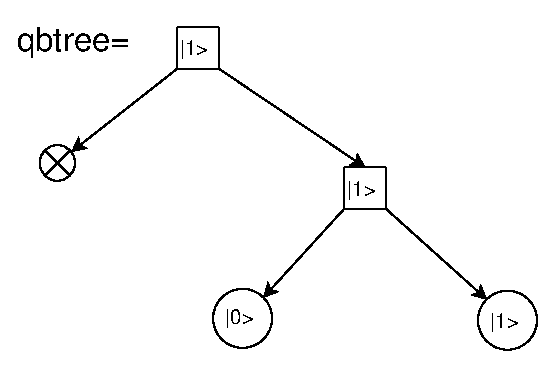
\includegraphics[scale=.6]{images/treeExample.eps}
\end{center}
\caption{Pictorial representation of \inlqpl{qbtree}}\label{fig:treeExample}
\end{figure}
\begin{figure}[htbp]
\begin{center}
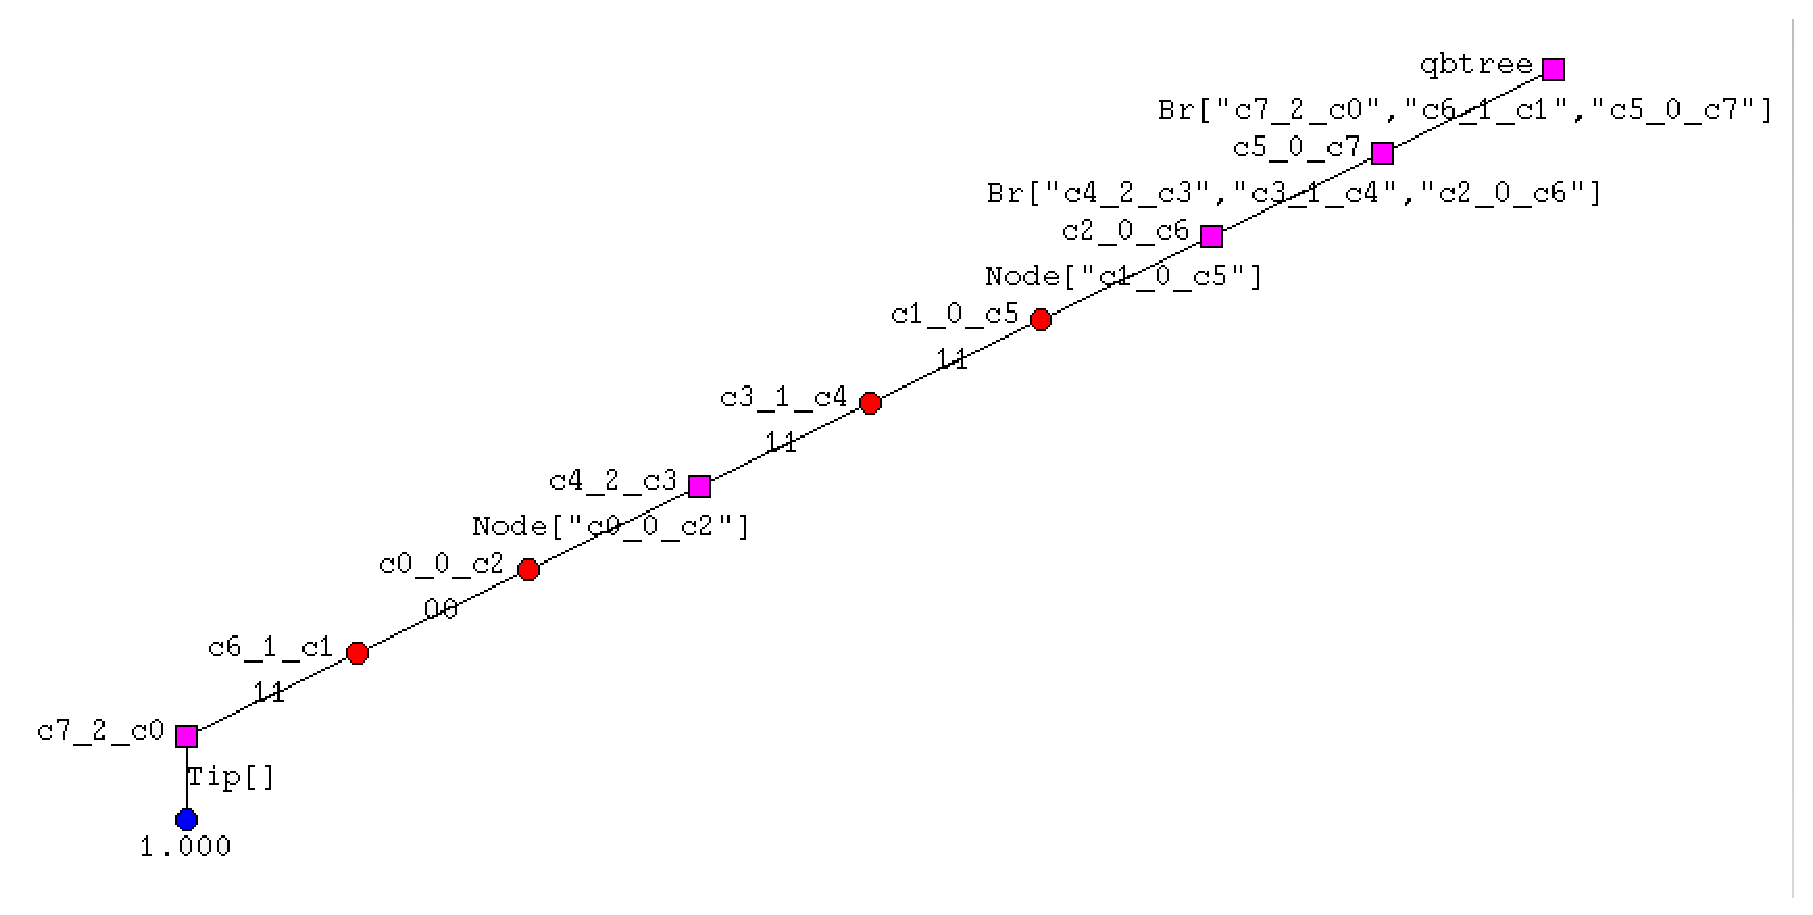
\includegraphics[scale=.5]{images/treeExampleInQS.eps}
\end{center}
\caption{Quantum stack contents after creation of \inlqpl{qbtree}}\label{fig:treeExampleInQS}
\end{figure}
The assignment statement which creates \inlqpl{qbtree} uses five constructor
expressions. The second assignment statement, which creates 
\inlqpl{intlist} uses six constructor expressions and one function expression.
% The extent of the constructor expressions are shown by the underlines here.
% {\begin{multline*}\footnotesize
%\shoveleft{\mathtt{qbtree =} 
%\underline{\mathtt{Br(}\underline{\mathtt{Tip}}\mathtt{,\ket{1},}
%\underline{\mathtt{Br(}\underline{\mathtt{Node(\ket{0})}}
%\mathtt{,\ket{1},}
%\underline{\mathtt{Node(\ket{1})}})})}; }\\
%\shoveleft{\mathtt{intlist =} 
%\mathtt{reverse(}\underline{\mathtt{Cons(5,}
%\underline{\mathtt{Cons(4,}
%\underline{\mathtt{Cons(3,}
%\underline{\mathtt{Cons(2,}
%\underline{\mathtt{Cons(1,}
%\underline{\mathtt{Nil}}\mathtt{)}}\mathtt{)}}\mathtt{)}}\mathtt{)}}\mathtt{)}}\mathtt{)};}
%\end{multline*}
% }

Constructor expressions either have no arguments
 (e.g. \inlqpl{Tip}, \inlqpl{Nil} above), or
require a parenthesized list of expressions which agree in both
number and type with the template supplied at the declaration of the
type. These expressions are unrestricted otherwise. They may be constants,
identifiers, other constructor expressions, expression calls or compound
expressions. Any expressions that are classical in nature, such as constants,
are upgraded to quantum automatically.

\subsection{Function expressions}\label{subsec:expressioncalls}
When a function returns a single value, it may be used in a
function expression. The bottom two lines of listing below shows
two examples of function expressions. 
\begin{lstlisting}
      f ::(c1:Int,c2:Int, c3:Int | q1:Qbit, i1:Int ; out:Qbit)
      = { ... }
      ...
         qout = f(c1,c2,c3 | q1,i2);
	 qlist = Cons(f(1,2,3 | qout, 5),Nil);
\end{lstlisting}
In the first function expression, \inlqpl{f} is the right hand side of 
an assignment statement. The assignment statement
 creates the variable \inlqpl{qout}
with the value returned by the function.

In the second function expression, \inlqpl{f} is the first argument of a 
constructor expression which will create a one element \inlqpl{List(Qbit)}.
The constructor expression is part of an assignment statement which
creates the variable \inlqpl{qlist} and sets it to
the one element list. Note that due to linearity, the variable 
\inlqpl{qout} is no longer available after the second function expression.

A function expression is always a quantum expression, so it may only be
used in those places where quantum expressions are allowed. Nesting of
these calls inside constructor expressions, other function expressions
and function calls is allowed.

\begin{figure}[htbp]
\lstinputlisting[style=linqpl]{examplecode/append.qpl}
\caption{\lqpl{} code for appending two lists}\label{fig:appendtwolists}
\end{figure}

In \vref{fig:appendtwolists}, line \ref{line:append:funcexp} shows the 
\inlqpl{append} being used as a function expression inside of a
constructor expression.
